\documentclass[runningheads,a4paper]{llncs}

\usepackage{amssymb}
\setcounter{tocdepth}{3}
\usepackage{graphicx}
\usepackage{algorithmic}

\usepackage{url}
\urldef{\mailsa}\path|{adrianr, davidc, jayen, bernhardh}@cse.unsw.edu.au|  
\newcommand{\keywords}[1]{\par\addvspace\baselineskip
\noindent\keywordname\enspace\ignorespaces#1}

\begin{document}

\mainmatter

\title{Fast Object Detection on a Resource Limited Robot}

% a short form should be given in case it is too long for the running head
\titlerunning{Fast Object Detection}

\author{Adrian Ratter \and David Claridge\and \\
    Jayen  Ashar \and Bernhard Hengst}

\authorrunning{Vision Stuff}

\institute{School of Computer Science and Engineering,\\
University of New South Wales, UNSW Sydney 2052 Australia}

%
% NB: a more complex sample for affiliations and the mapping to the
% corresponding authors can be found in the file "llncs.dem"
% (search for the string "\mainmatter" where a contribution starts).
% "llncs.dem" accompanies the document class "llncs.cls".
%

\toctitle{Fast Object Detection on a Resource Limited Robot}
\tocauthor{Adrian Ratter}
\maketitle


\begin{abstract}
\emph{abstract} environment.
Accurate visual object identification is a vital requirement for the operation of most autonomous robots. In many cases, computational resources limit the complexity of algorithms that can be used to run in real time. We describe a set of algorithms that use a combination of downsampled colour based object identification and high resolution edge detection to provide the basis for the visual perception of an Aldebaran Nao robot on a RoboCup soccer field. Optimised to run in real time on an autonomous robot, these techniques can potentially be applied to other resource limited domains.
\end{abstract}

\section{Introduction}

Automatic identification of objects in a video feed is a significant research area in robotics, and forms the major component of most robot’s sensory perception of the world. One application of this research area is in the Robocup Standard Platform League. Robocup is an annual soccer competition where teams of 3 Aldebaran Nao robots play compeltely autonomous games. Each robot has two cameras in its head (although only one can be used at a time), with the computation performed on its AMD Geode processor.

However, while the structured area of a soccer field permits the use of algorithms tailored for the identification of specific objects, such as orange balls, coloured goals, field lines and other robots, a game of soccer played using the Nao robots presents specific and complex challenges in the field of computer vision, including: \begin{itemize}
\item{The vision processing system has to run fast enough to provide up-to-date information for other systems, such as localisation, locomotion and behavoural planning to process. This means frames should be able to be processed at 30 frames per second}
\item{It is required to run in real time on the Nao's 500MHz processor}
\item{Objects must be identified accurately enough to allow kinematics to provide reasonable estimates of their distance away from the robot}
\item{It must be robust enough to perform with a high level of image blurring}
\item{It must identify false positives as little as possible}
\item{It must be robust enough to handle a significant amount of object occlusion}
\end{itemize}

The main contribution of the paper is an efficient set of algorithms that use virtual saccades to provide both efficiency and accuracy. The algorithm uses a hybrid of colour calibration on downsampled frames to provide fast identification of approximate areas of objects such as goals and balls, and edge detection on areas of interest in the full resolution image to allow the positions of these objects to be found very accurately, with a substantial amount of robustness to uneven and changing lighting conditions. Additionally, we present a novel method that uses the field edge and the field lines to provide updates to the robot's current estimated position on the field.

In the rest of this paper we will describe how the downsampled frames are used to initially identify possible locations of the various objects on the field. We then show how this enables us to use virtual saccades to perform edge detection in small areas of the high resolution image, enabling us to achieve the often competing goals of high accurcy and high efficiency. Finally, we will show how the field edge and field lines identified in the downsampeld image can be used to aid in the localisation of the robot.

This approach was implemented for the 2010 RoboCup Standard Platform League in Singapore, for both the technical challenges and the soccer tournmament. The University of New South Wales (UNSW) placed first in the technical challenges and second in the soccer competition against 23 other international teams.

\section{Saliency Scan}

In order to achieve our goal of identifying areas of interest in the image as fast as possible, the first step of the rUNSWift vision pipeline is to subsample the image down to a 160x120 pixel resolution, and store a colour classified version of this image.

The colours are colour calibrated offline using a weighted kernel classification algorithm developed for previous Robocup competitions \cite{kimcuongpham}. In this, each training sample increases a weighting for that particular YUV value toward the classified colour. Neighbouring values in colour-space, within a fixed Euclidean radius, also have their weights increased, at an exponentially decreasing rate, giving generalisation. The kernel file can then be used to generate a constant-time lookup table for use on the robot at runtime. The main colours calibrated are orange (the ball), green (the field), white (the field lines and parts of the robots), yellow (the yellow goals), red (the pink band worn by robots on the red team) and blue (the blue goals and the blue band worn by robots on the blue team).

We will describe in the following sections how the colour calibrated saliency scan can be used to rapidly identify objects of interest in the image. In addition, while the saliency scan is being genrated, histograms in the x and y-axes for each of the major field-space colours are generated. The maxima of these histograms can be found efficiently, allowing the rest of the vision system to analyse only the most interesting parts of the image at the native resolution.

Mention the goal detection here? Or in its own section, and just reference here. ALso should the efficiency optimisations that were performed to make the saliency scan faster talked about here?

\section{Field Edge Detection and Use in Localisation}

To further reduce the amount of the image that has to be processed for object identification, and to assist with localisation, the edges of the green field are detected using the Saliency Scan image. In 2009 B-Human used a convex hull algorithm to exclude areas above the field edge \cite{thomas09code}, which achieves the first goal of reducing the area of the image to be processed. In 2010 rUNSWift used a similar method of vertical scanning to detect points on the edge of the field, but rather than a convex hull algorithm, multiple iterations of the RANSAC algorithm was used to find straight lines. When two field edge lines are detected, the possible positions of the robot are reduced to 4 hypotheses.

\begin{figure}
\centering
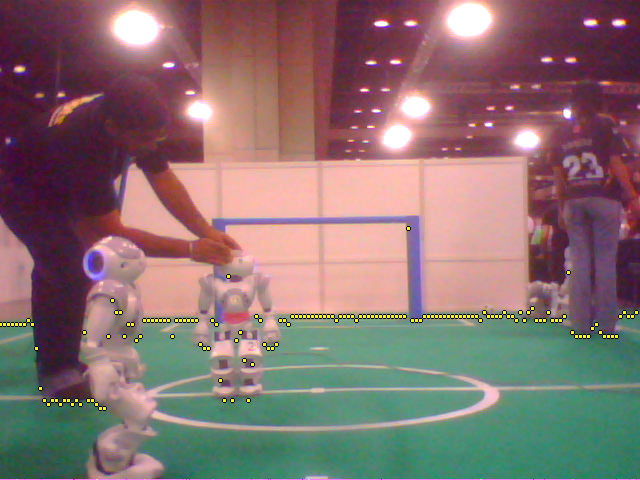
\includegraphics[width=1.0\textwidth]{figures/EdgeDetection_OneLinePoints}
\caption{Candidate points for a field-edge line} \label{fig:EdgeDetection_OneLinePoints}
\end{figure}

Initially the first green pixel in each column of the saliency scan is recorded, by scanning vertically from the horizon (the horizon is found by using kinematics to take into account the robot's current joint angles) down. See \ref{fig:EdgeDetection_OneLinePoints}.

Secondly, the RANSAC algorithm chooses the parameters for a line in $t_1x + t_2y + t_3 = 0$ form, to maximise the number of points that fit a line. See \ref{fig:EdgeDetection_OneLinePointsAndLine}.

\begin{figure}
\centering
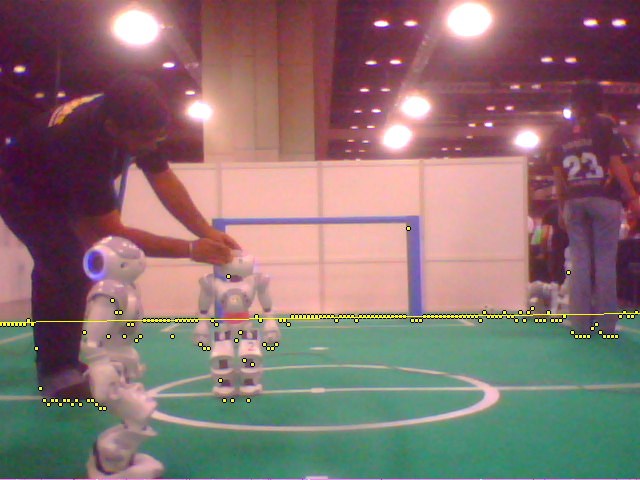
\includegraphics[width=1.0\textwidth]{figures/EdgeDetection_OneLinePointsAndLine}
\caption{Line found by performing RANSAC on the candidate points} \label{fig:EdgeDetection_OneLinePointsAndLine}
\end{figure}

Finally, the consensus set of the first line is removed from the candidate points, and RANSAC is repeated, possibly finding a second line. See \ref{fig:EdgeDetection_TwoLines}.

\begin{figure} [t]
\centering
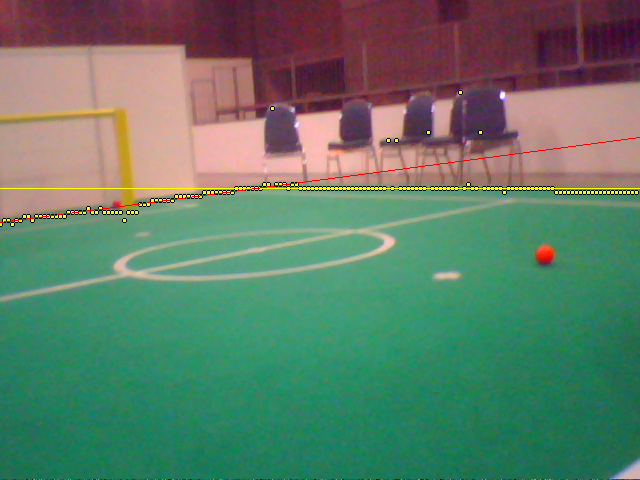
\includegraphics[width=1.0\textwidth]{figures/EdgeDetection_TwoLines}
\caption{Lines found by performing RANSAC twice on the candidate points} \label{fig:EdgeDetection_TwoLines}
\end{figure}

In addition to reducing the amount of the image to be scanned for objects to the parts of the image below the field edge, these field edge observations were able to be used to provide an update to the robot's current perceived position in the Kalman filter relative to either to goal line or the side line. One field-edge line generates an infinite set of hypotheses (see Figure \ref{figKFfieldEdgeUpdate}) for where the robot may lie, so we choose the field-edge closest (in terms of orientation) to our current position estimate.

\begin{figure} [ht]
\centering
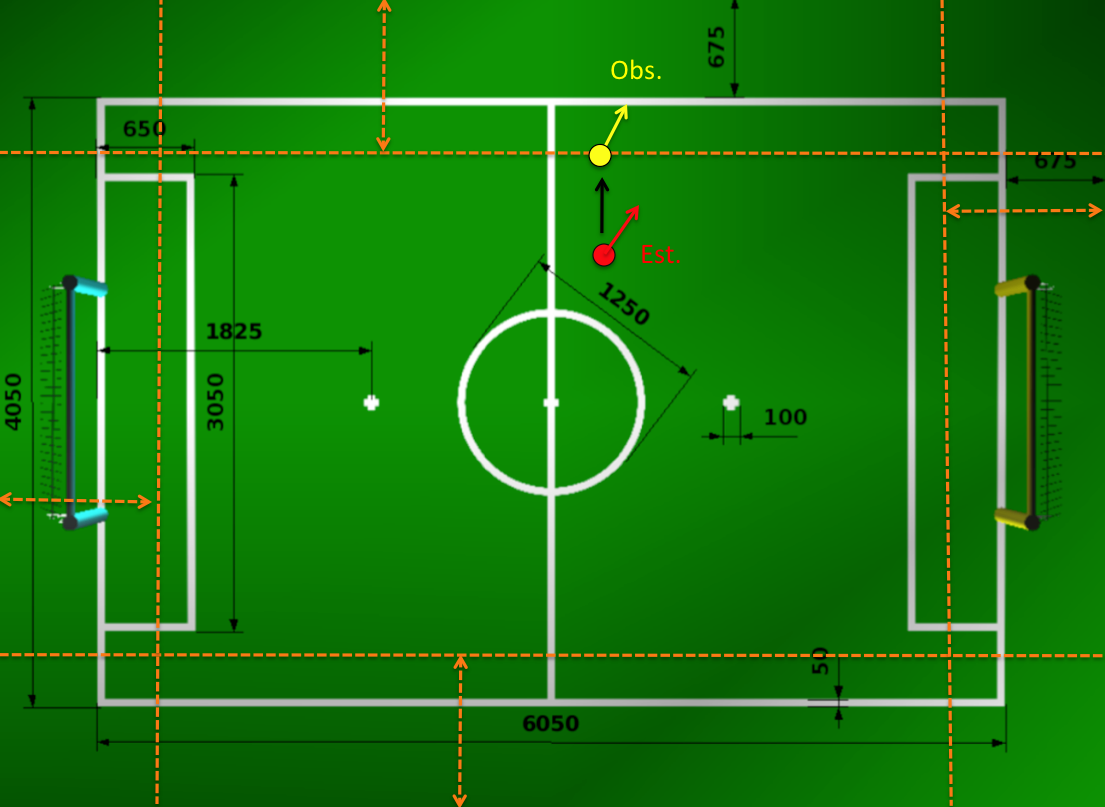
\includegraphics[width=0.8\textwidth]{figures/KFfieldEdgeUpdate}
\caption{Update from field-edge lines, illustrated on the field diagram\cite{RobocupRules}.} \label{figKFfieldEdgeUpdate}
\end{figure}

We require the expected orientation of the chosen field edge to be within 45 degrees of the observed orientation to perform an update. If this criteria is met, we then update the orientation and the distance away from the chosen field edge.

If two field edges are detected, this procedure is performed iteratively for each one, allowing one good observation to be used even when the other is a false-positive that fails the 45 degrees test. Because this whole procedure is heavily dependant on the current state estimate, only a local update to the current position can be performed using this information.

\section{Region Building Using the Saliency Scan}

We then scan the colour classified pixels underneath the field edge to identify potential areas, or regions, that could represent important features, such as the ball, other robots, or field lines. The contents of each of these regions are then analysed to determine what object they may represent, and potentially examined in more detail using the full resolution image to get object identification as accurate as possible. By only examining small areas of interest at the full resolution, this method of virtual saccades enabled us to greatly increase the runtime spped of the vision processing system.

This is achieved by scanning each column of the saliency scan image below the field edge to identify \emph{runs} of non-field green coloured pixels. For runs starting with orange (ball coloured) pixels, the run will finish when either a green, white, robot red or robot blue pixel is found, when a few unclassified pixels are found, or when the bottom of the image is reached. Alternatively, for runs starting with other colours, they will finish when either an orange pixel is found, when more than one green pixel in a row is found, or when the bottom of the image is reached. This distincation is made to make sure a region potentially containing a ball is not later joined to a region containing either a robot or a field line.

Once a run is finished, information about the run is used to build regions. A run is connected to an existing region only if the following conditions are met: \begin{itemize}
\item{If the last run added to the region is adjecent to the current run}
\item{If the region contains orange pixels, the run will only be connected if it also contains orange pixels. Similarly, if the region contains no orange pixels, the run will only be connected if it also contains no orange pixels. This test is to split potential ball regions from potential field line and robot regions}
\item{If the run contains robot coloured pixels and the region does not, they are only joined if the region is less than a certain width. This condition is used to separate regions containing robots and regions containing field lines touching the robot}
\item{If the run contains no robot coloured pixels and the region does, they are only joined if the difference between the x coordinate of the current run and the x coordinate of the right most robot coloured pixel in the region is less than a certain threshold. A larger threshold for the width is used if the run started at the field edge. As with the last condition, this is used to stop robots and field lines from being combined into the same region}
\item{If the length of the run if between half the average run length of the region so far and double the average run length of the region so far. This is a further condition to separate regions containing robots and regions containing field lines}
\end{itemize}
If all these conditions are met, the run is connected to the region. However, if no region is able to meet all these conditions, a new region is created for the run. An array of pointers to regions containing runs from the previous column is stored to avoid large numbers of regions slowing down processing. If the next run to be potentially combined is in the same column as the previous run, the search through this array for potential regions can start where the previous search finished because the next run will always be further down the image than the current run. This process also allows regions to be combined if a run that can be accepted into both regions is encountered. This processing is summarised in the following algorithm:

\begin{algorithmic}
    \FORALL{$column\ \mathbf{in}\ saliencyScan$}
    \FORALL{$row\ \mathbf{in}\ column$}
    \IF{have reached the end of a $run$}
    \FOR{$reg\ \mathbf{in}\ lastColumnRegions$}
    \IF{$reg.startY > run.endY$} 
    \STATE{\bf{continue}}
    \ENDIF
    \IF{$reg.endY \ge run.startY$}
    \IF{conditions for joining $run$ to $reg$ are met}
    \IF{$run$ hasn't been joined to a region yet}
    \STATE{Join $run$ to $reg$}
    \STATE{Add $reg$ to end of $thisColumnRegions$}
    \ELSE
    \STATE{Merge $reg$ with previous region $run$ joined}
    \ENDIF
    \ENDIF
    \ELSE
    \STATE{$\mathbf{remove}\ reg$ from $lastColumnRegions$} 
    \ENDIF
    \ENDFOR
    \IF{$run$ has not been joined to a region}
    \STATE{Create new region for $run$}
    \STATE{Add new region to $thisColumnRegions$}
    \ENDIF
    \ENDIF
    \ENDFOR
    \STATE{Set $lastColumnRegions\ =\ thisColumnRegions$}
    \STATE{Set $thisColumnRegions.size\ =\ 0$}
    \ENDFOR
\end{algorithmic}

An example of the output of the region detection is shown in Figure \ref{fig:RegionBuilder1}.

\begin{figure} [t]
\centering
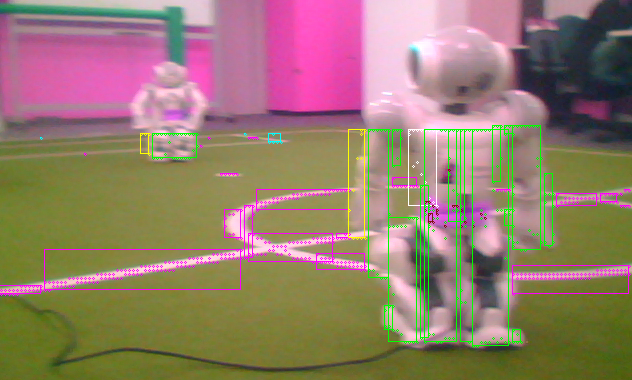
\includegraphics[width=0.7\textwidth]{figures/regionScreenshot1.png}
\caption{Regions identified during the region detection process} \label{fig:RegionBuilder1}
\end{figure}

Throughout this process, information about each run is collected in region it joins, allowing information such as the number of pixels of each colour in the region, the coordinates of the bounding box of the region, the average length of the runs in the regions, the start and end coordinates of each run in the region, and the bounding box of the robot colours in the region to be stored. This information is then used to identify what object (if any) the region is most likely to contain so the region can be examined in more detail for a specific object.

The initial object classification is performed by examining the colours, shape and location of each region to determine if the region is more likely to contain a ball, field line, robot, or just be noise, such as noise from an error in the field edge. As orange coloured regions are grown seperately from other regions, any regions containing orange pixels are considered to be potential balls. Other regions require more detailed classification than a simple examiniation of the colours contained in the region as a single robot can potentially cover many regions, some of which may consist of only white pixels, and thus appearing very similar to regions containing lines. In order to deal with this problem, regions adjacent a region containing either robot red or robot blue coloured pixels, or a region that starts at the field edge and contains runs of a similar length (in some cases the red and blue identifying band of a robot may be above the field edge, and the colour information from the band is not contained in the region) are examined to see if they should be merged together. This decision is largely made by looking at the dimensions of the bounding box of the region (if it is taller than it is wide, it is more likely to be part of a robot, and less likely to be a field line), the extent of overlap between the two regions, and the average length of the runs in a region. Any regions remaining that are not identified as possible balls, possible robots, or noise (such as very small regions, or regions touching the field edge) are considered to be field lines.

\section{Image Edge Detection}

The often used technique of pre-calibrating the colours that appear on a Robocup field can be quite unreliable and prone to degredation due to lighting changes since the calibration was performed. Additionally, it can be difficult to fully cover the range of colours an object can appear as on the field, often due to the range of intensities of shadows or the curvature of objects such as the ball. In previous Robocup events, rUNSWift have noticed a degradation in the ability to both detect balls and to accurately determine their position as more people stand around the field to watch the game.

An alternative to a colour calibration approach is to use edge detection to find the outline of objects. Unfortunately, common edge detection methods to identify all the edges in the image, such as Hough transforms, are computationally too expensive to run in real time on the Nao's, before considering the additional challenge of complex shape identification. A hybrid solution of these two methods was therefore used to combine the accuracy and robustness of edge detection with the computational speed of colour calibration to identify both balls and the goal posts. The hybrid solution involved firstly using colours to quickly identify potential locations, and then edge detection to perform accurate and reliable identification

\subsection{Ball Detection}

In terms of ball detection, edge detection can be used around the location a region that has been identified as a probable ball to find a list of pixels on the edge of the ball. A circle is then fitted to these points to allow the location of the ball to be accurately determined. Rows and columns of the full resolution image are scanned outwards from the region until the \emph{v} channel of adjacent pixels differs by more than a certain threshold. Only the \emph{v} channel was used in the ball edge detection as the brightness of the ball tends to change quite markedly near the edge of the ball, causing edge to often be detected inside the ball when a combination of \emph{y, u} and \emph{v} channels was used. In order to further increase the efficiency of this method, the space between rows and columns scanned for edges was adjusted according to the size of the region to ensure that balls close to the robot didn't take too long to process, but balls far away from the robot could still be properly identified.

Once pixels around the edge of a ball have been identified, a circle can be quickly fitted to these points by randomly selecting 3 edge pixels, and finding the interesection of the perpendicular bisectors of the lines joining the three points. The interesction gives the centre of the ball, and the distance between the intersection and any of the 3 pixels gives the radius of the ball. If this process is repeated several times and the median of the centre and radius measurements is taken, any small erros in the edge detection are greatly reduced.

Figure \ref{fig:ballDetection} shows an example of the edge detection being used to accurately identify a ball. The left hand image shows the colour calibrated image, where it can be seen that a substantial part of the ball is unclassified (note that unclassified colours appear as light blue in the screenshot). The right hand image however shows that the edge detection has enabled the edge of the ball to be precisely located. This is particuarly important for ball detection as kicks need to be lines up very precisely for them to work well.

\begin{figure} [t]
\centering
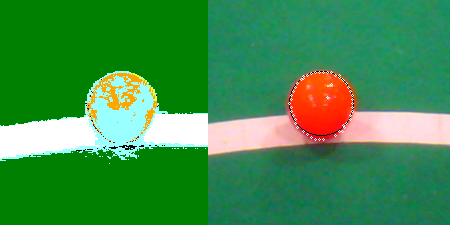
\includegraphics[width=0.7\textwidth]{figures/ballDetectionScreenshot.png}
\caption{A screenshot of the ball detection. The left image shows the colour calibrated image, while the right shows the edge points identified and the circle fitted to the edge points} \label{fig:ballDetection}
\end{figure}

\subsection{Goal Detection}

As the majority of the goals appear above the field edge, goals are not identified during the region building. Instead, the histograms generated while the saliency scan is being built are used to identify the likely approximate positions of the goals, and edge detection is then used to find the exact position of the goal posts, or to remove false positives from the histogram stage.

This is achieved by firstly finding the maximum value in the y-axis histogram for one of the goal colours.  Only one y coordinate is used because if there are 2 goal posts in the image, they will occupy approximately the same y coordinate range, and the maximum in the histogram will most likely occur at a y coordinate occupied by both posts. The x-axis histogram is then scanned to find local maximums above a certain threshold for the goal colour. To avoid several local maximums being detected in the same goal post, the histogram value of the goal post colour has to decrease to be at least 3 times less than the maximum value before another local maximum can be recorded. The same proceedure is used for both goal colours.

Several horizontal and vertical scan lines are used around each pair of x and y coordinates identified using the histograms. Each scan starts around the pair of x and y coordinates, and continues outwards until an edge is detected. For goal detection, an edge is found when the two pixels differ in the sum of the differences in the \emph{y, u} and \emph{v} values by more than a certain threshold. All channels are used as the colour of the background around the goal posts cannot be controlled, so any significant change in any channel needs to be registered as an edge. These scan lines result in a rectangle representing the goal post, which can then be used by the localisation algorithms.

Do i need info about the sanity checks here?

\section{Robot Detection}

Robot detection is a useful ability during the Robocup tournament as it has the potential to allow smarter behaviour in moving away from opposing robots and passing to friendly robots. Additionally, in the 2010 Robocup competition, one of the additional challenges required a robot to dribble around stationary robots and score a goal without touching any of the robots.

Much of the work to identify the location of robots is performed in the region builder to identify areas in the image that could possibly represent robots. As robots are fairly large, and their position does not need to be as accurately determined as the ball, only the saliency scan was used for detection. As previously mentioned, it is possible for some possible robot regions to not contain any robot colours due to the band being above the field edge, as seen in Figure \ref{fig:robotDetection}. In these cases, the area immediately above the robot region is scanned to find pixels classified as one of the robot band colours. A few sanity checks are then performed to reduce the number of false positives, such as removing regions that are entirely below the field edge, or removing regions that are smaller than a minimum width.

\begin{figure} [t]
\centering
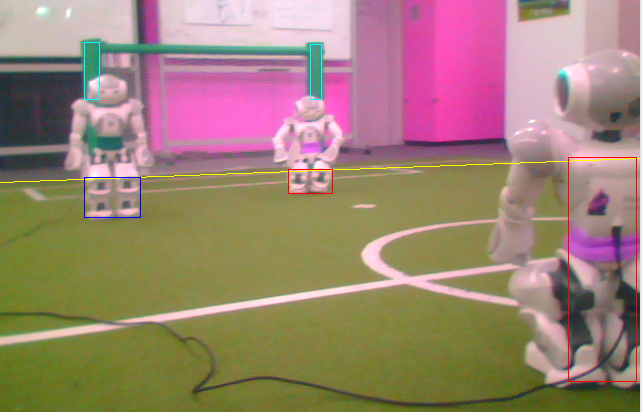
\includegraphics[width=0.7\textwidth]{figures/robotDetectionScreenshot.png}
\caption{The bounding box around robot regions identified in the image} \label{fig:robotDetection}
\end{figure}

\section{Field Lines and Use in Localisation}

As previously mentioned, regions contain a list of the start and end coordinates of each \emph{run} in the region. As runs are a vertical sequence of non-green classified pixels, the start and end coordinates of each run in regions identified as containing field lines can be used as the edge points of field lines. In directly using the information generated during the region building process, the field line detection can run extremely fast. If each of these coordinates are converted to a distance and angle away from the robot using kinematics, they can be used to determine the likelihood of a robot being in a given position by examining how well the points match a map of the field lines if the robot were in that position.

The map of the field is precomputed and stored as a binary file. It contains a grid of the field at a resolution of 1cm. Each entry in the grid is given the value of the distance squared from that point in the field to the closest field line (including the centre circle and penalty spots). A visualisation of this map is shown in Figure \ref{fig:fieldDistancesMap}. 

\begin{figure} [t]
\centering
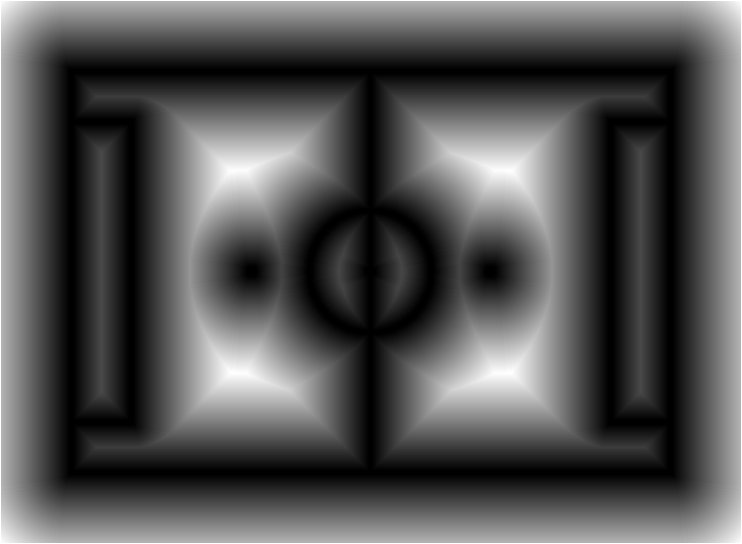
\includegraphics[width=0.7\textwidth]{figures/fieldDistancesMap.png}
\caption{A map of the field line distances, where the lighter the shading, the further away the point is from a field edge} \label{fig:fieldDistancesMap}
\end{figure}

A telescoping search is performed around the robot's previous estimated position to find the best estimate of its current position. At each stage of the search, the likelihood of being in the given position is determined by scanning through the list of field line points, offsetting the points by the position, and determining the entry in the grid that each point corresponds to. The average of each of these entries is taken to be the likelihood of being at that position. In each iteration of this search, the resolution of the possible positions is reduced to give an accurate, yet fast result. An example of a good match using this algorithm are shown in Figure \ref{fig:fieldLineMatching}. The searches have a small amount of intertia to slightly penalise matches away from the starting position to discourage the returned location drifting when the match is constant along one axis, such as when only one field line is seen. The result is used as a local update to the localisation Kalman filter.

\begin{figure} [t]
\centering
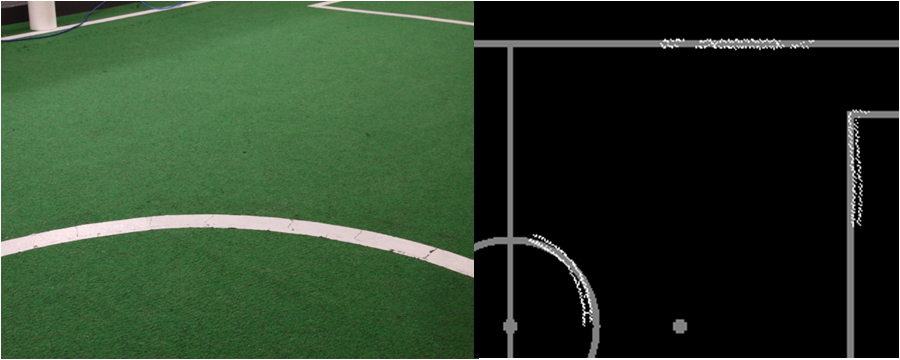
\includegraphics[width=0.7\textwidth]{figures/fieldLineMatching.png}
\caption{An example of a match achieved using the telescoping search} \label{fig:fieldLineMatching}
\end{figure}

\section{Performance in RoboCup}

The set of algorithms presented in this paper formed the cornerstone of UNSW's visual object identification for the 2010 RoboCup competition. In this competition, rUNSWift placed second in the overall compeition, and first in the rechnical challenges against 23 other international teams. In particular, it was able to successfully handle the difficult conditions of a final game where people crowded around the field can pose significant challenges for affecting the lighting and creating false positives, without noticeable degradation in performance. In testing before the competition, we found that vision was able to run at approximately 30 frames per second during game conditions.

As the region builder uses the field edge detection to only scan the image below the field edge, and field edges are used for localisation, field edge detection is a vital part of our vision system. We found that when the field edge(s) could be seen clearly, or with a few small obstructions, the field edge detection worked consistently and accurately. However, when there was a lot of obstruction, such as several robots, or a referee, the field lines were often mis-placed. At times this caused a noticeable deterioration in the localisation while lining up to make a kick for goals.

The advantage of using a hybrid approach of initial colour detection, and then accurate edge detection proved to be very beneficial to the performance of both the gaol detection and the ball detection. In following this method, only a very small number of pixels in the saliency scan needed to be the correct colour for the edge detection to give an accurate match. This allowed us to consistently and accurately detect the balls and goals, even from the opposite side of the field depite the large amount of colour variation due to the curved surfaces of the goals and the ball, and various shadows on the goals. In particular, we found that the virtual saccades did not prevent the ball from being detected at the far side of the field.

Robot detection was the least developed part of our vision infrastructure, and consequently tended to report false positives and false negatives at a significantly higher rate than other components of vision. That said, the robot detection was used unmodified in the Dribble Challenge (where our robot was required to dribble the ball around 3 stationary robots and score a goal without either our robot or the ball touching the robot obstacles), in which rUNSWift placed third, helping us to achieve first place in the technical challenges. While in the majority of circumstances the robot detection was able to correctly identify the presence of a robot and its colour, it was unable to report robots on opposite sides of the field due to not enough pixels of the team band colour in the saliency scan.

The field line detection part of the visual processing system was successful in providing information to the localisation algorithm. We found that it was able to provide very accurate local adjustments to the estimated position, which was particuarly useful when lining up before the start of play. We would like to extend this to be able to provide global localisation in the future.

\section{Related Work}

A number of alternate methods have been divised to solve the complex task of object identifiaction in the resource limited environment of RoboCup.

In order to limit the amount of interference from the background, it is often a useful first step to identify the edge of the field in the image. Any item above this edge can therefore be eliminated. The method used in \cite{thomas09code} to find the edge of the field is to scan down each column in the image to find a green segment of a minimum length, and fit a convex hull to the start of the green segments. We imagine this approach would make the position of the field edge more accurate when there are a lot of objects around the edge, however this would make it much more difficult to use field edges as part of localisation.

Due to the limited processing power available on the Nao's, it is not possible to scan every pixel in the image fast enough to run in real time. An interesting approach is taken in \cite{north2005object}, where the density of horizontal and vertical scan lines is changed depending on how close the scan lines are in the image to horizon. This uses the theory that objects close to the camera will be large enough to be seen using extremely low resolution scan lines, but objects further away, near the horizon, will appear much smaller, and therefore need a much higher density of scan lines in order to be detected. The drawback to this approach is that shape identification and repeated accesses are harder and slower. An alternate approach can be seen in \cite{von2004tracking}, where regions are grown from the green field; with the white field lines, robots and balls separating the green regions. They propose that, as the robot moves, the regions can be incrementally grown and shrunk, resulting in far fewer pixels needing to be processed and updated each frame. This idea of using previous frames to help lower the computation time of the current frame, while not explored in our 2010 vision system, is a worthwhile avenue for future research.

One of the most difficult parts of the object identification for robocup is the distinction between field lines and robots, as many parts of the robots are white or close to white. This means that some kind of processing, other than colour, has to be used to separate field lines and robots. The method used in \cite{thomas09code} to achieve this is to first create a series of small white coloured regions that could represent either parts of a line or parts of a robot. These regions are then analysed in terms of their shape, and ones that more likely represent robots are marked. Finally, areas of the images where there is a cluster of these marked regions are considered to most likely contain robots, and every region in this area is thus removed. However this method does not actually identify the robots.

The authors of \cite{rofer2004fast} propose a different of edges and colour to achieve fast object recognition. In this method, a grid of horizontal and vertical scan lines is used to search for pixels where there is a significant drop in the Y-channel compared to the previous pixels searched. As the field is generally darker than the field lines and the robots, this can indicate an edge between an object and the field. The pixels around this can then be colour classified to see if they are white or orange.

\section{Conclusion}

Arguably the most important form of sensory perception, a vision processing system must be highly
efficient, robust and accurate to enable it to perform accurately and reliably in the dynamic world
of a soccer game. By utilising a hybrid of colour classification and edge detection, we were able
to reliably identify robots, goals, field lines and balls during the 2010 Robocup competition. Our
approach of using sub-sampled images allowed us to reduce the processing of redundant data, and
achieve processing speeds of approximately 30 frames per second, while our use of edge detection
allowed the ball and goal detection to perform well in changing lighting conditions.

\begin{thebibliography}{4}

\bibitem{kimcuongpham} Pham, K.C.:Incremental learning of vision recognition using ripple down rules.
Honours Thesis. The University of New South Wales (2005)

\bibitem{thomas09code} R{\"o}fer, T., Laue, T., M{\"u}ller, J., B{\"o}sche, O., Burchardt, A., Damrose, E., Gillmann, K., Graf, C., Haas, T.J., H{\"a}rtl, A., Rieskamp, A., Schreck, A., Sieverdingbeck, I., Worch, J.H.:
B-Human Team Report and Code Release 2009, \url{http://www.b-human.de/index.php?s=publications} (2010)

\bibitem{RobocupRules} Soccer Rules for the RoboCup 2009 Standard Platform League Competition, \url{http://www.tzi.de/spl/pub/Website/Downloads/Rules2010.pdf} (2010)

\bibitem{north2005object} North, A.: Object recognition from sub-sampled image processing.
Honours Thesis. The University of New South Wales (2005)

\bibitem{von2004tracking} Von Hundelshausen, F., Rojas, R.: Tracking regions. In:
RoboCup 2003: Robot Soccer World Cup VII, pp.250--261. Springer (2004)

\bibitem{rofer2004fast} R\"{o}fer, T., J\"{u}ngel, M.: Fast and robust edge-based localization in the sony four-legged robot league. In: RoboCup 2003: Robot Soccer World Cup VII, pp262--273. Springer (2004)

\end{thebibliography}

\end{document}
